% --- Manual DA-method legend used by Figures \ref{fig:catch22-importance}
% and \ref{fig:cumsum-disc}.  The original ICML legend.eps only contains
% colour markers; its gnuplot wrapper has the text labels commented out,
% so we render the legend natively in LaTeX with matching colours.
\providecolor{daASC}{RGB}{31,67,142}
\providecolor{daDif}{RGB}{67,144,196}
\providecolor{daFAA}{RGB}{154,194,222}
\providecolor{daIma}{RGB}{86,179,180}
\providecolor{daKoV}{RGB}{152,200,140}
\providecolor{daLA}{RGB}{222,188,84}
\providecolor{daTTS}{RGB}{233,150,98}
\providecolor{daTDD}{RGB}{215,72,75}
\providecolor{daVaD}{RGB}{171,28,30}
\newcommand{\daLegMark}[2][0.9pt]{\textcolor{#2}{\rule[1.6pt]{1.2em}{#1}}}
\newcommand{\daLegItem}[2]{\daLegMark{#1}\,#2}
\newcommand{\daLegItemBold}[2]{\daLegMark[1.7pt]{#1}\,\textbf{#2}}
\newcommand{\daLegendBlock}{%
  {\small\centering
   \daLegItemBold{daASC}{ASCENSION}\hspace{1.0em}%
   \daLegItem{daDif}{Diffusion-TS}\hspace{1.0em}%
   \daLegItem{daFAA}{FAA}\hspace{1.0em}%
   \daLegItem{daIma}{ImagenTime}\hspace{1.0em}%
   \daLegItem{daKoV}{KoVAE}\par
   \daLegItem{daLA}{LA}\hspace{1.0em}%
   \daLegItem{daTTS}{TTS-GAN}\hspace{1.0em}%
   \daLegItem{daTDD}{Time-DDPM}\hspace{1.0em}%
   \daLegItem{daVaD}{VaDE}\par}%
}

\section{Experiments}
\label{sec:experiments}

In this section, we evaluate ASCENSION against leading state-of-the-art DA methods to validate our central hypothesis
that progressively exploring under-represented latent regions and
expanding the initial data distribution improves DA, particularly
under distribution discrepancies.

\subsection{Experimental setup}
\label{sec:setup:experimental}

% REVISED FOR TMLR (dataset selection fix)
We use the UCR Archive of 128 univariate TSC datasets (see \tablename~\ref{app:datasets}), retaining 102 of the 128.
We exclude 15 datasets with missing values or variable lengths, 4
datasets with single-instance classes, and 7 further datasets that
were left out of the original experimental campaign and are kept out
for comparability across all methods.


Following \citep{fawaz2019deep}, which identifies ResNet-50 and
FCN (Fully Convolutional Network) as top UCR performers, we use these architectures as in
\citep{koonce2021resnet50, scabini2023networks}. We also evaluate
Moment \citep{goswami2024moment}, a transformer-based multi-task
foundation model pretrained on the UCR training splits (excluding
test splits). We apply ASCENSION to augment the training data and
assess whether augmentation still helps an encoder that has
already seen this data. As the test splits are held out from
Moment's pretraining, any test-set improvement reflects a performance benefit.
% ADDED FOR TMLR (rebuttal C5/WS9)
Moment also probes a distinct regime: the classifier is a frozen
foundation-model encoder with a shallow head, so synthetic samples
cannot reshape the learned features and can only move the decision
boundary.

We compare ASCENSION to nine related DA methods: one traditional
(FAA) and eight generative (VaDE, TTS-GAN, KoVAE, Time-DDPM, LA,
ImagenTime, Diffusion-TS, MODALS; see Section~\ref{sec:setup:gen-da}
and Figure~\ref{fig:SoTa} for details). FAA provides a classical baseline,
while KoVAE, VaDE, and MODALS share architectural traits with
ASCENSION. Diffusion-TS, ImagenTime, LA, Time-DDPM, and TTS-GAN
are recent generative baselines. As MODALS' public code is
defunct and unmaintained, we benchmark it on the HAR dataset from
\citep{cheung2020modals} instead of UCR.


% REVISED FOR TMLR (rebuttal C1)
\tablename~\ref{tab:main-results} reports every method under a
single fixed hyperparameter configuration, applied uniformly across
all 102 datasets and repeated over three independent runs. ASCENSION
uses $\alpha = 1.5$, one augmentation iteration, and uniform loss
weights ($\gamma_1 = \gamma_2 = \gamma_3 = \gamma_4 = 1$), while
baselines use their authors' recommended defaults. The complementary
analysis with ASCENSION at its best per-dataset configuration is
given in Appendix~\ref{app:best-config}.
% ADDED FOR TMLR (rebuttal C7)
As the UCR archive provides no validation split, model selection
follows the best-epoch-on-test convention standard in the UCR
literature~\citep{fawaz2019deep}. We apply this rule identically to
every method and to the no-augmentation baseline in every ResNet and
FCN experiment, so absolute accuracies are optimistic for every
method. Moment uses a single deterministic fit with no epoch-based
selection.
% ADDED FOR TMLR (rebuttal Q2)
All methods use the same generation budget, which follows the
empirical class distribution: at each iteration we draw
$|\mathcal{I}_y|$ candidate samples per class $y$, one per real
sample, $n$ in total.
Baselines add all $n$ candidates to the training set, doubling it,
whereas ASCENSION keeps only the candidates that pass the
Bayes-region filter and therefore adds fewer.



\subsubsection{Performance evaluation metrics}
\label{sec:results:metrics}

We rely on the UCR archive protocol~\citep{dau2019ucr} and use
classification accuracy as the primary metric, quantifying each
DA method's gain as the change in accuracy before and after
augmentation.
% REVISED FOR TMLR (rebuttal C1)
\tablename~\ref{tab:main-results} reports the number of datasets with
improved, unchanged, or worsened accuracy, along with the mean
accuracy change over each subset, both given as mean (std) over the
three runs. Full results appear in Appendix~\ref{app:per_dataset}.

\subsubsection{Performance comparison analysis}
\label{sec:results:main}

% REVISED FOR TMLR (rebuttal C1): fixed-configuration table over three runs
% replaces the best-per-dataset-configuration table, now Appendix tab:best-config.
\begin{table}[t]
\centering
\caption{Main comparison under a \emph{single fixed hyperparameter
configuration} per method ($\alpha = 1.5$, one iteration for ASCENSION;
authors' recommended defaults for the baselines), applied uniformly across
all 102 UCR datasets and all three classifiers, over \textbf{three
independent runs}. Cells report the mean (std) over the three runs of the
number of datasets (out of 102) with improved, unchanged, or worsened
accuracy, of the mean accuracy change
$\overline{\Delta\mathrm{Acc}} = \mathrm{augmentation\_accuracy} -
\mathrm{base\_accuracy}$ over each subset, and of the net total over the
102 datasets. Arrows $(\uparrow, \downarrow)$ mark direction of
improvement; \textbf{bold} marks the best mean per column.}
\label{tab:main-results}
\resizebox{\textwidth}{!}{%
\begin{tabular}{@{}llrrrrrrr@{}}
\toprule
 & \multirow{2}{*}{\bf DA method} & \multirow{2}{*}{\bf (Venue, Year)}
  & \multicolumn{2}{c}{\bf Improved}
  & {\bf Unchanged}
  & \multicolumn{2}{c}{\bf Worsened}
  & {\bf Total} \\
  & &
  & $\uparrow$Nb$_{\text{data}}$ & $\uparrow\overline{\Delta\mathrm{Acc}}$
  & Nb$_{\text{data}}$
  & $\downarrow$Nb$_{\text{data}}$ & $\downarrow\overline{\Delta\mathrm{Acc}}$
  & $\overline{\Delta\mathrm{Acc}}$ \\
\midrule
\multirow{9}{*}{\rotatebox{90}{ResNet}}
 & VaDE & (IJCAI, 2016) & 37.3\,(7.6) & 2.4\,(0.3)\% & 26.0\,(14.7) & 38.7\,(10.5) & -3.9\,(2.8)\% & -0.75\,(1.33)\% \\
 & FAA & (NeurIPS, 2019) & 36.3\,(17.5) & 4.5\,(2.9)\% & 15.0\,(6.1) & 50.7\,(22.7) & -4.7\,(3.9)\% & -1.55\,(3.25)\% \\
 & TTS-GAN & (AIME, 2022) & 37.7\,(10.1) & 2.3\,(0.1)\% & 12.7\,(2.9) & 51.7\,(11.9) & -9.6\,(1.2)\% & -3.94\,(0.70)\% \\
 & KoVAE & (ICLR, 2024) & 43.3\,(4.6) & 1.9\,(0.3)\% & 15.7\,(3.5) & 43.0\,(2.6) & -2.7\,(0.5)\% & -0.32\,(0.04)\% \\
 & Time-DDPM & (SENS.\,J., 2023) & 40.7\,(6.4) & 7.7\,(7.4)\% & 6.0\,(5.3) & 55.3\,(9.0) & -11.1\,(8.8)\% & -3.49\,(3.28)\% \\
 & LA & (ArXiv, 2023) & 29.7\,(13.6) & 2.6\,(0.6)\% & 14.7\,(1.5) & 57.7\,(15.0) & -2.5\,(1.2)\% & -0.81\,(1.40)\% \\
 & ImagenTime & (NeurIPS, 2024) & 39.3\,(21.1) & 1.7\,(0.5)\% & 14.3\,(1.5) & 48.3\,(22.2) & -4.1\,(1.8)\% & -1.47\,(2.41)\% \\
 & Diffusion-TS & (ICLR, 2024) & 39.0\,(17.3) & 1.9\,(0.4)\% & 13.0\,(4.6) & 50.0\,(21.8) & -5.4\,(3.6)\% & -2.36\,(3.75)\% \\
 & \textbf{ASCENSION} &  & \textbf{59.0\,(4.4)} & 3.3\,(0.6)\% & 14.3\,(2.1) & \textbf{28.7\,(5.1)} & -2.2\,(0.4)\% & \textbf{+1.30\,(0.39)\%} \\
\midrule
\multirow{9}{*}{\rotatebox{90}{FCN}}
 & VaDE & (IJCAI, 2016) & 36.3\,(4.9) & 3.0\,(0.4)\% & 22.7\,(6.8) & 43.0\,(2.0) & -4.4\,(2.2)\% & -0.81\,(0.81)\% \\
 & FAA & (NeurIPS, 2019) & 23.7\,(14.2) & 5.2\,(1.8)\% & 11.7\,(7.8) & 66.7\,(20.8) & -6.7\,(7.2)\% & -4.08\,(6.48)\% \\
 & TTS-GAN & (AIME, 2022) & 32.3\,(4.7) & 2.5\,(0.3)\% & 13.0\,(4.6) & 56.7\,(7.8) & -9.6\,(1.2)\% & -4.61\,(1.47)\% \\
 & KoVAE & (ICLR, 2024) & 38.0\,(4.4) & 2.6\,(0.4)\% & 14.3\,(0.6) & 49.7\,(4.7) & -2.9\,(0.6)\% & -0.43\,(0.33)\% \\
 & Time-DDPM & (SENS.\,J., 2023) & 22.0\,(18.0) & 9.2\,(7.8)\% & 6.3\,(4.7) & 73.7\,(13.3) & -15.2\,(6.0)\% & -7.58\,(1.81)\% \\
 & LA & (ArXiv, 2023) & 37.7\,(6.5) & 2.7\,(0.4)\% & 15.3\,(3.2) & 49.0\,(9.2) & -2.5\,(0.2)\% & -0.18\,(0.20)\% \\
 & ImagenTime & (NeurIPS, 2024) & 39.3\,(3.2) & 2.8\,(0.1)\% & 12.7\,(3.8) & 50.0\,(2.6) & -3.3\,(0.3)\% & -0.52\,(0.08)\% \\
 & Diffusion-TS & (ICLR, 2024) & 38.0\,(3.5) & 3.4\,(0.3)\% & 12.7\,(4.2) & 51.3\,(7.0) & -6.5\,(6.2)\% & -2.24\,(3.79)\% \\
 & \textbf{ASCENSION} &  & \textbf{47.0\,(4.4)} & 3.3\,(0.4)\% & 17.0\,(3.6) & \textbf{38.0\,(4.6)} & -2.6\,(1.0)\% & \textbf{+0.55\,(0.52)\%} \\
\midrule
\multirow{9}{*}{\rotatebox{90}{Moment}}
 & VaDE & (IJCAI, 2016) & 34.0\,(1.7) & 2.2\,(0.6)\% & 12.7\,(4.2) & 55.3\,(4.0) & -3.3\,(1.9)\% & -1.11\,(0.93)\% \\
 & FAA & (NeurIPS, 2019) & 50.3\,(1.5) & 5.3\,(2.2)\% & 4.0\,(1.7) & 47.7\,(2.1) & -7.2\,(4.2)\% & -0.68\,(0.73)\% \\
 & TTS-GAN & (AIME, 2022) & 34.0\,(6.1) & 2.5\,(0.8)\% & 9.7\,(6.4) & 58.3\,(6.7) & -4.1\,(2.1)\% & -1.51\,(1.22)\% \\
 & KoVAE & (ICLR, 2024) & 27.3\,(1.5) & 3.4\,(0.3)\% & 4.3\,(0.6) & 70.3\,(1.5) & -6.7\,(4.5)\% & -3.71\,(3.04)\% \\
 & Time-DDPM & (SENS.\,J., 2023) & 31.7\,(3.1) & 2.8\,(0.8)\% & 5.3\,(2.5) & 65.0\,(3.0) & -5.2\,(1.5)\% & -2.43\,(0.45)\% \\
 & LA & (ArXiv, 2023) & 32.3\,(2.3) & 3.8\,(1.2)\% & 4.0\,(2.0) & 65.7\,(1.2) & -6.1\,(0.6)\% & -2.68\,(0.09)\% \\
 & ImagenTime & (NeurIPS, 2024) & 29.7\,(4.5) & 2.8\,(0.7)\% & 9.3\,(2.5) & 63.0\,(7.0) & -4.2\,(1.7)\% & -1.84\,(1.65)\% \\
 & Diffusion-TS & (ICLR, 2024) & 26.7\,(2.3) & 2.7\,(0.7)\% & 8.7\,(4.0) & 66.7\,(4.9) & -5.1\,(3.2)\% & -2.68\,(2.06)\% \\
 & \textbf{ASCENSION} &  & \textbf{54.3\,(6.7)} & 3.4\,(0.4)\% & 9.3\,(2.1) & \textbf{38.3\,(4.9)} & -2.7\,(0.5)\% & \textbf{+0.83\,(0.26)\%} \\
\bottomrule
\end{tabular}%
}
\end{table}

% REVISED FOR TMLR (rebuttal C1/C2)
\tablename~\ref{tab:main-results} shows that no baseline reaches a
positive three-run mean total on any classifier: 0 of the 27
baseline method-classifier cells are positive, and across individual
runs the baselines end positive in only 7 of their 72 classifier-run
combinations, with no single baseline exceeding 3 of its 9. The
strongest baselines stay slightly below zero, KoVAE at
$-0.32\,(0.04)\%$ on ResNet, LA at $-0.18\,(0.20)\%$ on FCN, and FAA
at $-0.68\,(0.73)\%$ on Moment. Time-DDPM pairs the highest mean
gains on its winning datasets ($7.7\%$ ResNet, $9.2\%$ FCN) with
severe drops on the rest ($-11.1\%$, $-15.2\%$), yielding heavily
negative totals. ASCENSION is the only method whose three-run mean
total is positive on each classifier ($+1.30\,(0.39)\%$ ResNet,
$+0.55\,(0.52)\%$ FCN, $+0.83\,(0.26)\%$ Moment), and its total is
positive in 8 of its 9 classifier-run combinations, the exception
being FCN run 3 at $-0.03\%$. ASCENSION also shows the highest mean
count of improved datasets (59.0, 47.0, 54.3) and the lowest mean
count of degraded datasets on every classifier (28.7 ResNet, 38.0
FCN, 38.3 Moment, against 38.7--57.7, 43.0--73.7, and 47.7--70.3 for
the baselines), while its mean drop on degraded datasets stays below
$3\%$ throughout. These totals are modest in absolute terms, so we
next characterise how the gains are distributed across datasets
rather than claiming uniform improvement.

% ADDED FOR TMLR (rebuttal C2)
\tablename~\ref{tab:gain-distribution} details the distribution of
ASCENSION's per-dataset gains, run by run. The median gain is
moderate on ResNet ($+0.32\%$ to $+0.84\%$ across runs), zero on FCN
in all three runs, and between $0.00\%$ and $+1.03\%$ on Moment,
while between 58 and 79 of the 102 datasets are non-negative in
every run. The gains are concentrated: the three largest per-dataset
gains carry $24$--$36\%$ of the net total on ResNet, $30$--$66\%$ on
Moment, and $67$--$74\%$ on FCN in the two runs where the net total
is far enough from zero. FCN is therefore the weak case: the median
dataset gains nothing in all three runs, one run ends at $-0.03\%$,
and the gains are the most concentrated. On FCN, ASCENSION is better
described as a low-risk method than as one that helps in general,
while ResNet is the favourable case and Moment sits in between.

\begin{table}[t]
\centering
\small
% ADDED FOR TMLR (rebuttal C2)
\caption{Distribution of ASCENSION's per-dataset accuracy gains
under the fixed configuration, run by run: median gain,
interquartile range (IQR), number of datasets whose absolute change
is within one accuracy point, and number of datasets with a
non-negative change, out of 102.}
\label{tab:gain-distribution}
\begin{tabular}{@{}llrrrr@{}}
\toprule
\textbf{Classifier} & \textbf{Run} & \textbf{Median (\%)} & \textbf{IQR (\%)}
  & \textbf{Within 1 pt} & \textbf{Non-negative} \\
\midrule
\multirow{3}{*}{ResNet}
  & 1 & $+0.65$ & $3.21$ & 35 & 72 \\
  & 2 & $+0.32$ & $3.14$ & 39 & 69 \\
  & 3 & $+0.84$ & $3.09$ & 39 & 79 \\
\midrule
\multirow{3}{*}{FCN}
  & 1 & $0.00$ & $1.38$ & 59 & 63 \\
  & 2 & $0.00$ & $2.56$ & 44 & 69 \\
  & 3 & $0.00$ & $2.41$ & 43 & 60 \\
\midrule
\multirow{3}{*}{Moment}
  & 1 & $0.00$ & $3.15$ & 41 & 58 \\
  & 2 & $+1.03$ & $5.10$ & 22 & 67 \\
  & 3 & $+0.35$ & $3.96$ & 31 & 66 \\
\bottomrule
\end{tabular}
\end{table}

% ADDED FOR TMLR (rebuttal C4)
The per-dataset standard deviation of ASCENSION's gain across runs
has a median of $1.6$ (ResNet), $1.6$ (FCN), and $2.1$ (Moment)
accuracy points but reaches roughly $20$ points on individual
datasets (full table in Appendix~\ref{app:per-dataset-std}), so we
report distributions and ranks rather than single per-dataset
values.


In \tablename~\ref{tab:modals}, we compare ASCENSION to MODALS on the
HAR dataset, as UCR benchmarking is not feasible for MODALS (see
Section~\ref{sec:setup:experimental}). Using MODALS improves
baseline accuracy by $3.23\%$, while ASCENSION achieves a $4.78\%$
improvement over the baseline. 

\begin{table}[t]
\centering
\small
\caption{ASCENSION and MODALS performance on HAR dataset from
\citep{cheung2020modals}.}
\label{tab:modals}
\begin{tabular}{lccc}
\toprule
\textbf{Method} & \textbf{ASCENSION} & \textbf{MODALS} & \textbf{No Aug} \\
\midrule
Accuracy (\%) & $\mathbf{93.42}$ & $91.87$ & $88.64$ \\
\bottomrule
\end{tabular}
\end{table}

% ADDED FOR TMLR (rebuttal C3)
\subsubsection{Statistical significance}
\label{sec:results:significance}

We assess significance with the Friedman test followed by a Nemenyi
post-hoc analysis at the $5\%$ level ($k = 9$ methods, $N = 102$
datasets, critical difference $\mathrm{CD} = 1.19$), applied
separately to each of the nine classifier-run combinations. The
Friedman test is significant in all nine combinations, with the
largest $p$-value at $1.1 \times 10^{-6}$. ASCENSION obtains the
best mean rank in 8 of the 9 combinations, with per-run mean ranks
of $3.04$--$3.56$ on ResNet, $3.96$--$4.06$ on FCN, and
$3.62$--$3.75$ on Moment. In the ninth combination (FCN run 3),
Diffusion-TS leads by $0.10$, well inside the critical difference.
Beyond the critical difference, ASCENSION separates from 7--8 of the
8 baselines on ResNet, from 2 of 8 on FCN, and from 4--5 of 8 on
Moment, and it is never significantly worse than any competitor.
Figures~\ref{fig:cd-resnet-main}, \ref{fig:cd-fcn-main}, and
\ref{fig:cd-moment-main} show the critical-difference diagrams
computed on per-dataset accuracies averaged over the three
fixed-configuration runs, where ASCENSION reaches mean ranks of
$2.67$ (ResNet), $3.56$ (FCN), and $3.20$ (Moment).

% ADDED FOR TMLR (rebuttal C3)
\begin{figure}[t]
\centering
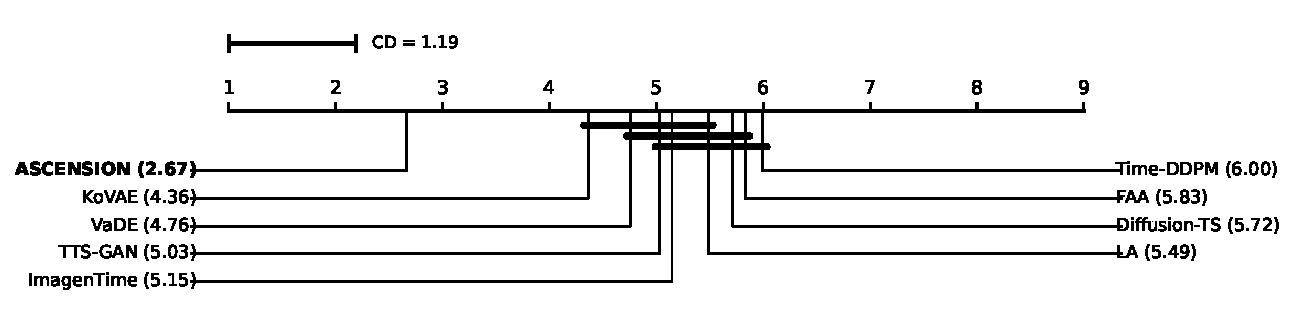
\includegraphics[width=0.85\linewidth]{figures/cd_diagram_resnet_fixedconfig.pdf}
\caption{Critical-difference diagram (Nemenyi post-hoc test, $5\%$
level) for ResNet, computed on per-dataset accuracies averaged over
the three fixed-configuration runs.}
\label{fig:cd-resnet-main}
\end{figure}

% ADDED FOR TMLR (rebuttal C3)
\begin{figure}[t]
\centering
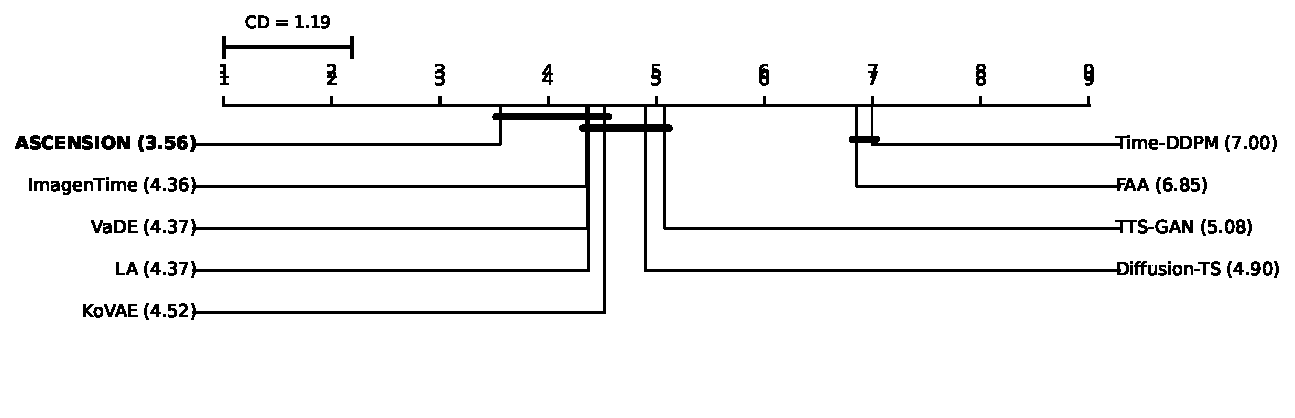
\includegraphics[width=0.85\linewidth]{figures/cd_diagram_fcn_fixedconfig.pdf}
\caption{Critical-difference diagram (Nemenyi post-hoc test, $5\%$
level) for FCN, computed on per-dataset accuracies averaged over the
three fixed-configuration runs.}
\label{fig:cd-fcn-main}
\end{figure}

% ADDED FOR TMLR (rebuttal C3)
\begin{figure}[t]
\centering
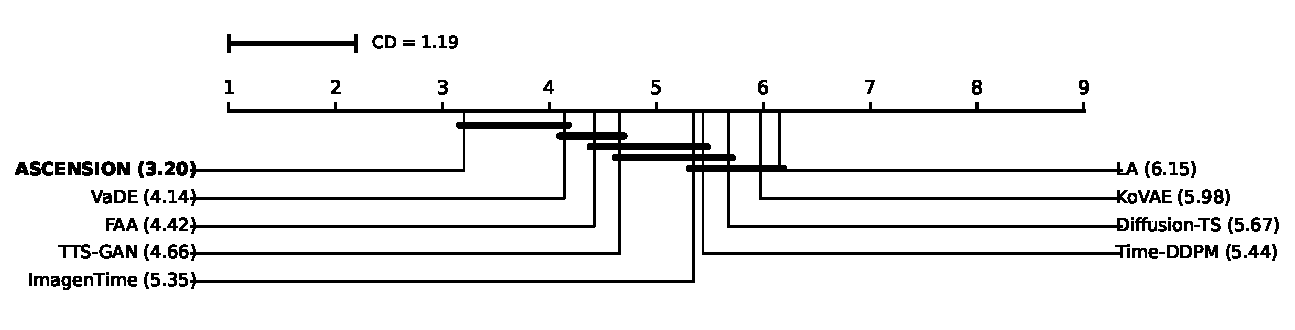
\includegraphics[width=0.85\linewidth]{figures/cd_diagram_moment_fixedconfig.pdf}
\caption{Critical-difference diagram (Nemenyi post-hoc test, $5\%$
level) for Moment, computed on per-dataset accuracies averaged over
the three fixed-configuration runs.}
\label{fig:cd-moment-main}
\end{figure}

% ADDED FOR TMLR (rebuttal WS8/Q4)
\subsubsection{Applicability profile}
\label{sec:results:applicability}

To characterise where ASCENSION helps, we group the 102 datasets by
their number of training samples per class and report the median
gain per group, with each dataset's gain averaged over the three
fixed-configuration runs (\tablename~\ref{tab:gain-by-group}). The
32 smallest datasets carry $39\%$, $84\%$, and $70\%$ of the net
total on ResNet, FCN, and Moment respectively. The overall
correlation between gain and samples per class is weak and not
significant (Spearman $\rho = -0.16$, $-0.05$, $-0.11$ with
$p = 0.10$, $0.63$, $0.27$), yet the smallest group's mean gain is
positive in all nine classifier-run combinations, ranging from
$+0.2$ to $+2.7$ points. Gain correlates positively with class
count: Spearman $\rho = +0.18$ ($p = 0.063$) on ResNet, $+0.22$
($p = 0.029$) on FCN, and $+0.23$ ($p = 0.019$) on Moment. Datasets
with at least 15 classes ($n = 7$) show median gains of $+2.1$,
$+4.6$, and $+1.6$ points, against $+1.0$, $0.0$, and $-0.1$ for
two-class datasets ($n = 39$). The benefit is clearest on ResNet and
Moment, on FCN only the smallest group is positive, and above 50
samples per class ASCENSION is close to neutral everywhere.
Appendix~\ref{app:gain-vs-spc} shows the per-dataset scatter of gain
against samples per class.

% ADDED FOR TMLR (rebuttal WS8)
\begin{table}[t]
\centering
\small
\caption{Median ASCENSION gain (accuracy points) per group of
training samples per class, with each dataset's gain averaged over
the three fixed-configuration runs.}
\label{tab:gain-by-group}
\begin{tabular}{@{}lrrrr@{}}
\toprule
\textbf{Samples per class} & $n$ & \textbf{ResNet} & \textbf{FCN} & \textbf{Moment} \\
\midrule
Fewer than 20 & 32 & $+1.65$ & $+0.24$ & $+2.07$ \\
20 to 49      & 23 & $+0.96$ & $-0.39$ & $+0.38$ \\
50 or more    & 47 & $+0.42$ & $+0.13$ & $+0.35$ \\
\bottomrule
\end{tabular}
\end{table}

\subsubsection{Embedded classifier performance}
\label{sec:results:embedded}

\tablename~\ref{tab:main-results} reports the \emph{default}
ASCENSION configuration: an external classifier (ResNet, FCN, or
Moment) is trained on the \emph{decoded} synthetic samples.
ASCENSION's training objective also includes an auxiliary
classifier head $\mathcal{L}_{\text{class}}$ on the latent code
(Section~\ref{sec:method:vae}), which enables two alternative
configurations that bypass the decoder.
\emph{ASCENSION$_{\text{Emb}}$} uses only this internal classifier
head, with no external classifier.
\emph{ASCENSION$_{c}$}, with $c \in \{\text{ResNet}, \text{FCN}\}$,
attaches an external classifier directly to the latent space
(after encoder and reparameterisation) rather than to the decoder
output. \tablename~\ref{tab:embedded} reports both alternative
configurations; the ablation studies in
Section~\ref{sec:analysis:ablation} use
ASCENSION$_{\text{ResNet-Emb}}$ and ASCENSION$_{\text{FCN-Emb}}$.
For the embedded variants, augmentation gain is defined as the
accuracy difference between the best of
ASCENSION$_{\text{Emb}}$ and ASCENSION$_{c}$ and the no-DA
baseline:
\begin{equation}
\mathrm{Acc}_{\text{Emb},c}
= \max_{k \in \{\text{Emb}, c\}} \mathrm{Acc}_{\text{ASCENSION}_{k}}
  - \mathrm{Acc}_{\text{base}}.
\end{equation}

\begin{table}[H]
\centering
\small
\caption{Number of datasets with improved, unchanged, or worsened
accuracy per DA for each embedded classifier; mean accuracy
change ($\uparrow\overline{\Delta\mathrm{Acc}}$) per category.
Arrows ($\uparrow, \downarrow$) show value preference.}
\label{tab:embedded}
\begin{tabular}{@{}lrrrrrrrr@{}}
\toprule
\multirow{2}{*}{\textbf{Embedded Classifier}}
  & \multicolumn{2}{c}{\bf Improved}
  & \multicolumn{2}{c}{\bf Unchanged}
  & \multicolumn{2}{c}{\bf Worsened}
  & \multicolumn{2}{c}{\bf Total} \\
  & $\uparrow$Nb$_{\text{data}}$ & $\uparrow\overline{\Delta\mathrm{Acc}}$
  & Nb$_{\text{data}}$ & $\overline{\Delta\mathrm{Acc}}$
  & $\downarrow$Nb$_{\text{data}}$ & $\downarrow\overline{\Delta\mathrm{Acc}}$
  & Nb$_{\text{data}}$ & $\overline{\Delta\mathrm{Acc}}$ \\
\midrule
ASCENSION$_{\text{Emb}}$         & 66 & 1.9\% & 12 & 0\% & 24 & \textbf{-1.6\%} & 102 & $+0.8\%$ \\
ASCENSION$_{\text{ResNet-Emb}}$  & \textbf{76} & \textbf{3.7\%} & 12 & 0\% & 14 & -5.7\% & 102 & $\mathbf{+2.1\%}$ \\
ASCENSION$_{\text{FCN-Emb}}$     & 60 & 2.9\% & 28 & 0\% & 14 & -1.7\% & 102 & $+1.2\%$ \\
\bottomrule
\end{tabular}
\end{table}

\tablename~\ref{tab:embedded} shows
ASCENSION$_{\text{ResNet-Emb}}$ yields the highest gain ($3.7\%$
on 76 datasets) with the largest drop ($-5.7\%$ on 14).
ASCENSION$_{\text{Emb}}$ is steadier ($1.9\%$ gain, $-1.6\%$
drop), while ASCENSION$_{\text{FCN-Emb}}$ offers moderate gains
($2.9\%$) with balanced trade-offs. Overall, ResNet yields the
largest gains but is less stable; FCN and the default classifier are
more consistent.

% -----------------------------------------------------------------
% NOTE — the cVAE comparison subsection (table + discussion)
% and the macro-$F_1$ subsection previously sat here; both moved
% to the appendix (Appendix~\ref{app:cvae_baseline}, Appendix~\ref{app:f1})
% for the TMLR resubmission to keep §4 focused on headline
% experimental results.
% -----------------------------------------------------------------



% =====================================================================
% ADDED FOR TMLR (additional analysis; AE points: model selection and
% the conditions under which the method is expected to perform well).
% Validation-selected iteration count under a fully sealed protocol.
% =====================================================================
\subsection{Selecting the iteration count without touching the test set}
\label{sec:results:valselect}

The comparisons above run every method under one fixed configuration,
and the hyperparameter study of
Section~\ref{sec:analysis:ablation} selects the best setting
per dataset retrospectively. A practitioner must instead choose the
iteration count from training data alone. We therefore evaluate a
deployment rule that selects the number of augmentation iterations per
dataset by internal validation, under a protocol in which the test set
is never consulted for any choice.

\paragraph{Protocol}
We reimplemented the generation pipeline from scratch and evaluate the
rule on the 78 UCR datasets whose training sets admit a stratified
internal validation fold (smallest class at least 10 samples, at least
30 training samples). Of these, 75 belong to the 102 datasets used
above, and the remaining three (the Cricket family) meet the criteria
but were not part of the original campaign. For each dataset and each
of three seeds, a validation fold is split from the training set,
synthetic samples are anchored on the remaining fit fold only, and we
train one classifier per rung of a ladder of $t \in \{0, 1, 2, 4, 8\}$
cumulative iterations. Each iteration retrains the VAE on the union of
the real fit fold and the previously accepted synthetic samples,
following Algorithm~\ref{alg:ascension}, while the Bayes-region filter
is evaluated by a verifier trained on real data only, so the
acceptance region cannot drift with the synthetic data. All early
stopping uses the validation fold. The deployed count $t^{*}$
maximises validation accuracy, with ties broken by validation
cross-entropy and then by the smaller $t$, and $t^{*} = 0$ deploys the
unaugmented baseline unchanged. Hypotheses, strata and the selection
rule were frozen before execution. Because every choice, training
epochs included, is made on the internal fold, absolute gains under
this sealed protocol are not comparable to
\tablename~\ref{tab:main-results} and are expected to be smaller. The
object of the analysis is the deployment rule. Full details are given
in Appendix~\ref{app:valselect}.

\begin{table}[H]
\centering
\caption{Deployed accuracy gain (points) of the validation-selected
iteration rule, over 78 UCR datasets and 3 seeds (234 cells per
classifier). Cell-level $t$ statistics in parentheses. The small-$n$
stratum (training sets of at most 60 samples, 11 datasets) was
pre-declared before execution. Abstention is the share of cells where
the rule deploys the unaugmented baseline ($t^{*}=0$).}
\label{tab:valselect}
\begin{tabular}{@{}lccc@{}}
\toprule
\bf Classifier & \bf All cells & \bf Small-$n$ stratum & \bf Abstention \\
\midrule
ResNet        & $+0.53$ $(t=1.83)$ & $+2.72$ $(t=2.59)$ & $49\%$ \\
FCN           & $+0.89$ $(t=2.95)$ & $+3.50$ $(t=2.59)$ & $48\%$ \\
InceptionTime & $+0.73$ $(t=2.66)$ & $-0.12$ $(t=-0.27)$ & $46\%$ \\
\bottomrule
\end{tabular}
\end{table}

\paragraph{Results}
\tablename~\ref{tab:valselect} reports the deployed gains for ResNet,
FCN and InceptionTime \citep{fawaz2020inceptiontime}. The rule
abstains on about half of the dataset-seed cells and, when it engages,
prefers small iteration counts (on ResNet, 41/29/32/18 engaged cells
at $t = 1/2/4/8$), consistent with the budget-matched control of
Appendix~\ref{app:budget-matched}. The deployed mean gain is positive
for all three classifiers, with cell-level $t$ statistics above 2.6
for FCN and InceptionTime, while for ResNet a per-dataset Wilcoxon
test does not separate the mean from zero ($p = 0.165$). The gains
concentrate where training data is scarce. On the pre-declared
small-$n$ stratum the deployed gain reaches $+2.72$ (ResNet) and
$+3.50$ (FCN) accuracy points, significant at the $5\%$ level, with
UMD ($+7.9$), BME ($+6.7$) and ArrowHead ($+5.3$) leading on ResNet.
The same stratum is flat for InceptionTime, whose small-$n$ baselines
average $86.1\%$ accuracy against $80.8\%$ for ResNet and $79.1\%$ for
FCN, and its gains appear instead on the remaining mid-sized datasets
($+0.97$, $t = 2.80$). This mirrors the applicability profile of
Section~\ref{sec:results:applicability}: augmentation pays where the
classifier still has headroom on scarce data, and a stronger inductive
bias moves that headroom, not the mechanism.

In summary, the validation-selected rule harms no stratum
systematically, abstains rather than harms where augmentation has
nothing to offer, and delivers its significant gains in the
small-training-set regime where augmentation has work to do. This
complements the fixed-configuration comparison with a rule a
practitioner can apply without touching the test set.

% ---------------------------------------------------------------------
% NOTE (Dorian): paragraphe hors-échantillon optionnel, à activer si tu
% veux montrer le test hors archive (honnête mais élargit la surface).
% ---------------------------------------------------------------------
% \paragraph{Out-of-archive probe}
% Applying the frozen rule unchanged to 11 datasets from the 2023
% bake-off collection that the project had never loaded yields a mean
% deployed delta of $-0.26$ points (median dataset $+0.20$), with the
% loss concentrated on two datasets whose internal validation
% systematically disagrees with their test split. The rule remains
% safe on 9 of the 11, and the failure mode is a property of the
% validation-test agreement, not of the generation step. We report
% this probe as a limitation of validation-based selection rather
% than as evidence for or against the augmentation itself.

\subsection{Ablation 1: Hyperparameter analysis \& tuning}
\label{sec:analysis:ablation}

We perform a unified ablation on
ASCENSION$_{\text{ResNet-Emb}}$ to assess key components and
hyperparameters:
(i) We sweep $\alpha \in \{1, \ldots, 5\}$ (with $\alpha = 1$
disabling scaling) and augmentation iterations
$\{1, \ldots, 9\}$ to study the $\alpha$-scaling mechanism and
performance gains evolution;
(ii) We test the effect of removing the clustering loss by
setting $\gamma_{3} = 0$;
(iii) We grid-search
$(\gamma_1, \gamma_2, \gamma_3, \gamma_4) \in G^{4}$, with
$G = \{1, 3, 5, 8, 10\}$, to find optimal loss-weighting. All
experiments use the protocol of
Section~\ref{sec:results:embedded}, isolating the impact of each
factor on classification accuracy.

\paragraph{$\alpha$-scaling mechanism ablation}
\tablename~\ref{tab:ablation} reports the accuracy improvements (Q1,
median, Q3, mean) observed for the full model and after removing the
$\alpha$-scaling mechanism across the 102 UCR datasets. Disabling
the $\alpha$-scaling mechanism leads to a notable drop in
performance, from $2.1\%$ to $0.09\%$ with
ASCENSION$_{\text{ResNet-Emb}}$, and from $1.2\%$ to $0.4\%$ with
ASCENSION$_{\text{FCN-Emb}}$.


\begin{figure}[!t]
\centering
\subcaptionbox{Step-wise accuracy degradation from clustering
loss removal.\label{fig:ablation-supp:cluster}}{%
\resizebox{0.46\textwidth}{!}{% GNUPLOT: LaTeX picture with Postscript
\begingroup
  \makeatletter
  \providecommand\color[2][]{%
    \GenericError{(gnuplot) \space\space\space\@spaces}{%
      Package color not loaded in conjunction with
      terminal option `colourtext'%
    }{See the gnuplot documentation for explanation.%
    }{Either use 'blacktext' in gnuplot or load the package
      color.sty in LaTeX.}%
    \renewcommand\color[2][]{}%
  }%
  \providecommand\includegraphics[2][]{%
    \GenericError{(gnuplot) \space\space\space\@spaces}{%
      Package graphicx or graphics not loaded%
    }{See the gnuplot documentation for explanation.%
    }{The gnuplot epslatex terminal needs graphicx.sty or graphics.sty.}%
    \renewcommand\includegraphics[2][]{}%
  }%
  \providecommand\rotatebox[2]{#2}%
  \@ifundefined{ifGPcolor}{%
    \newif\ifGPcolor
    \GPcolortrue
  }{}%
  \@ifundefined{ifGPblacktext}{%
    \newif\ifGPblacktext
    \GPblacktexttrue
  }{}%
  % define a \g@addto@macro without @ in the name:
  \let\gplgaddtomacro\g@addto@macro
  % define empty templates for all commands taking text:
  \gdef\gplbacktext{}%
  \gdef\gplfronttext{}%
  \makeatother
  \ifGPblacktext
    % no textcolor at all
    \def\colorrgb#1{}%
    \def\colorgray#1{}%
  \else
    % gray or color?
    \ifGPcolor
      \def\colorrgb#1{\color[rgb]{#1}}%
      \def\colorgray#1{\color[gray]{#1}}%
      \expandafter\def\csname LTw\endcsname{\color{white}}%
      \expandafter\def\csname LTb\endcsname{\color{black}}%
      \expandafter\def\csname LTa\endcsname{\color{black}}%
      \expandafter\def\csname LT0\endcsname{\color[rgb]{1,0,0}}%
      \expandafter\def\csname LT1\endcsname{\color[rgb]{0,1,0}}%
      \expandafter\def\csname LT2\endcsname{\color[rgb]{0,0,1}}%
      \expandafter\def\csname LT3\endcsname{\color[rgb]{1,0,1}}%
      \expandafter\def\csname LT4\endcsname{\color[rgb]{0,1,1}}%
      \expandafter\def\csname LT5\endcsname{\color[rgb]{1,1,0}}%
      \expandafter\def\csname LT6\endcsname{\color[rgb]{0,0,0}}%
      \expandafter\def\csname LT7\endcsname{\color[rgb]{1,0.3,0}}%
      \expandafter\def\csname LT8\endcsname{\color[rgb]{0.5,0.5,0.5}}%
    \else
      % gray
      \def\colorrgb#1{\color{black}}%
      \def\colorgray#1{\color[gray]{#1}}%
      \expandafter\def\csname LTw\endcsname{\color{white}}%
      \expandafter\def\csname LTb\endcsname{\color{black}}%
      \expandafter\def\csname LTa\endcsname{\color{black}}%
      \expandafter\def\csname LT0\endcsname{\color{black}}%
      \expandafter\def\csname LT1\endcsname{\color{black}}%
      \expandafter\def\csname LT2\endcsname{\color{black}}%
      \expandafter\def\csname LT3\endcsname{\color{black}}%
      \expandafter\def\csname LT4\endcsname{\color{black}}%
      \expandafter\def\csname LT5\endcsname{\color{black}}%
      \expandafter\def\csname LT6\endcsname{\color{black}}%
      \expandafter\def\csname LT7\endcsname{\color{black}}%
      \expandafter\def\csname LT8\endcsname{\color{black}}%
    \fi
  \fi
    \setlength{\unitlength}{0.0500bp}%
    \ifx\gptboxheight\undefined%
      \newlength{\gptboxheight}%
      \newlength{\gptboxwidth}%
      \newsavebox{\gptboxtext}%
    \fi%
    \setlength{\fboxrule}{0.5pt}%
    \setlength{\fboxsep}{1pt}%
    \definecolor{tbcol}{rgb}{1,1,1}%
\begin{picture}(3960.00,1512.00)%
    \gplgaddtomacro\gplbacktext{%
      \csname LTb\endcsname%%
      \put( 1200,440){\makebox(0,0)[r]{\strut{} \footnotesize  $-0.05$}}%
      \csname LTb\endcsname%%
      \put( 1200,610){\makebox(0,0)[r]{\strut{} \footnotesize  $-0.03$}}%
      \csname LTb\endcsname%%
      \put( 1200,781){\makebox(0,0)[r]{\strut{} \footnotesize  $-0.01$}}%
      \put(400,866){\makebox(0,0)[r]{\strut{}  \rotatebox{90}{\footnotesize Accuracy}}}%
      \put(600,866){\makebox(0,0)[r]{\strut{}  \rotatebox{90}{\footnotesize Improvement}}}%
      %\put(858,866){\makebox(0,0)[r]{\strut{}\rotatebox{90}{Acc. improvement)}}%
      \csname LTb\endcsname%%
      \put( 1200,951){\makebox(0,0)[r]{\strut{} \footnotesize  $0.01$}}%
      \csname LTb\endcsname%%
      \put( 1200,1122){\makebox(0,0)[r]{\strut{} \footnotesize  $0.03$}}%
      \csname LTb\endcsname%%
      \put( 1200,1292){\makebox(0,0)[r]{\strut{} \footnotesize  $0.05$}}%
      \put(1760,200){\makebox(0,0){\strut{} \footnotesize Step~$1$}}%
      \put(2350,200){\makebox(0,0){\strut{} \footnotesize Step~$2$}}%
      \put(2950,200){\makebox(0,0){\strut{} \footnotesize Step~$3$}}%
      \put(3550,200){\makebox(0,0){\strut{} \footnotesize Step~$4$}}%
      % \put(3563,220){\makebox(0,0){\strut{}  Step~$5$}}%
    }%
    \gplgaddtomacro\gplfronttext{%
    }%
    
    \gplbacktext
    \put(300,-120){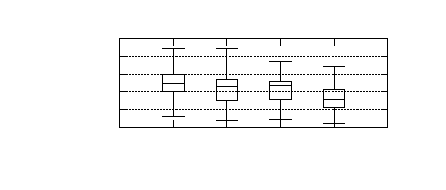
\includegraphics[width={210.00bp},height={90.60bp}]{images/cluster_as_boxplot}}%
    \gplfronttext
  \end{picture}%
\endgroup
}}\hfill
\subcaptionbox{Averaged accuracy variance per dataset over
$\gamma_i$. Smaller values imply low
impact.\label{fig:ablation-supp:gamma}}{%
\resizebox{0.46\textwidth}{!}{% GNUPLOT: LaTeX picture with Postscript
\begingroup
  \makeatletter
  \providecommand\color[2][]{%
    \GenericError{(gnuplot) \space\space\space\@spaces}{%
      Package color not loaded in conjunction with
      terminal option `colourtext'%
    }{See the gnuplot documentation for explanation.%
    }{Either use 'blacktext' in gnuplot or load the package
      color.sty in LaTeX.}%
    \renewcommand\color[2][]{}%
  }%
  \providecommand\includegraphics[2][]{%
    \GenericError{(gnuplot) \space\space\space\@spaces}{%
      Package graphicx or graphics not loaded%
    }{See the gnuplot documentation for explanation.%
    }{The gnuplot epslatex terminal needs graphicx.sty or graphics.sty.}%
    \renewcommand\includegraphics[2][]{}%
  }%
  \providecommand\rotatebox[2]{#2}%
  \@ifundefined{ifGPcolor}{%
    \newif\ifGPcolor
    \GPcolorfalse
  }{}%
  \@ifundefined{ifGPblacktext}{%
    \newif\ifGPblacktext
    \GPblacktexttrue
  }{}%
  % define a \g@addto@macro without @ in the name:
  \let\gplgaddtomacro\g@addto@macro
  % define empty templates for all commands taking text:
  \gdef\gplbacktext{}%
  \gdef\gplfronttext{}%
  \makeatother
  \ifGPblacktext
    % no textcolor at all
    \def\colorrgb#1{}%
    \def\colorgray#1{}%
  \else
    % gray or color?
    \ifGPcolor
      \def\colorrgb#1{\color[rgb]{#1}}%
      \def\colorgray#1{\color[gray]{#1}}%
      \expandafter\def\csname LTw\endcsname{\color{white}}%
      \expandafter\def\csname LTb\endcsname{\color{black}}%
      \expandafter\def\csname LTa\endcsname{\color{black}}%
      \expandafter\def\csname LT0\endcsname{\color[rgb]{1,0,0}}%
      \expandafter\def\csname LT1\endcsname{\color[rgb]{0,1,0}}%
      \expandafter\def\csname LT2\endcsname{\color[rgb]{0,0,1}}%
      \expandafter\def\csname LT3\endcsname{\color[rgb]{1,0,1}}%
      \expandafter\def\csname LT4\endcsname{\color[rgb]{0,1,1}}%
      \expandafter\def\csname LT5\endcsname{\color[rgb]{1,1,0}}%
      \expandafter\def\csname LT6\endcsname{\color[rgb]{0,0,0}}%
      \expandafter\def\csname LT7\endcsname{\color[rgb]{1,0.3,0}}%
      \expandafter\def\csname LT8\endcsname{\color[rgb]{0.5,0.5,0.5}}%
    \else
      % gray
      \def\colorrgb#1{\color{black}}%
      \def\colorgray#1{\color[gray]{#1}}%
      \expandafter\def\csname LTw\endcsname{\color{white}}%
      \expandafter\def\csname LTb\endcsname{\color{black}}%
      \expandafter\def\csname LTa\endcsname{\color{black}}%
      \expandafter\def\csname LT0\endcsname{\color{black}}%
      \expandafter\def\csname LT1\endcsname{\color{black}}%
      \expandafter\def\csname LT2\endcsname{\color{black}}%
      \expandafter\def\csname LT3\endcsname{\color{black}}%
      \expandafter\def\csname LT4\endcsname{\color{black}}%
      \expandafter\def\csname LT5\endcsname{\color{black}}%
      \expandafter\def\csname LT6\endcsname{\color{black}}%
      \expandafter\def\csname LT7\endcsname{\color{black}}%
      \expandafter\def\csname LT8\endcsname{\color{black}}%
    \fi
  \fi
    \setlength{\unitlength}{0.0500bp}%
    \ifx\gptboxheight\undefined%
      \newlength{\gptboxheight}%
      \newlength{\gptboxwidth}%
      \newsavebox{\gptboxtext}%
    \fi%
    \setlength{\fboxrule}{0.5pt}%
    \setlength{\fboxsep}{1pt}%
    \definecolor{tbcol}{rgb}{1,1,1}%
\begin{picture}(3960.00,1512.00)%
    \gplgaddtomacro\gplbacktext{%
      \csname LTb\endcsname%%
      \put(330,600){\makebox(0,0)[r]{\strut{}\footnotesize$0$}}%
      \csname LTb\endcsname%%
      \put(330,832){\makebox(0,0)[r]{\strut{}\footnotesize$3$}}%
      \csname LTb\endcsname%%
      \put(330,1095){\makebox(0,0)[r]{\strut{}\footnotesize$6$}}%
      \put(130,885){\makebox(0,0)[r]{\strut{}\rotatebox{90}{\footnotesize Frequency}}}%
      \csname LTb\endcsname%%
      \put(330,1360){\makebox(0,0)[r]{\strut{}\footnotesize$9$}}%
      \put(581,300){\makebox(0,0){\strut{}\footnotesize0}}%
      % \put(701,220){\makebox(0,0){\strut{}0.004215}}%
      % \put(820,220){\makebox(0,0){\strut{}0.007025}}%
      % \put(939,220){\makebox(0,0){\strut{}0.009815}}%
      % \put(1058,220){\makebox(0,0){\strut{}0.0126}}%
      % \put(1178,220){\makebox(0,0){\strut{}0.015449999999999998}}%
      % \put(1297,220){\makebox(0,0){\strut{}0.018299999999999997}}%
      \put(1416,300){\makebox(0,0){\strut{}\footnotesize0.02}}%
      % \put(1535,220){\makebox(0,0){\strut{}0.023899999999999998}}%
      % \put(1655,220){\makebox(0,0){\strut{}0.0267}}%
      % \put(1774,220){\makebox(0,0){\strut{}0.0295}}%
      % \put(1893,220){\makebox(0,0){\strut{}0.0323}}%
      % \put(2013,220){\makebox(0,0){\strut{}0.0351}}%
      % \put(2132,220){\makebox(0,0){\strut{}0.0379}}%
      \put(2251,300){\makebox(0,0){\strut{}\footnotesize0.04}}%
      \put(2000,100){\makebox(0,0){\strut{}\footnotesize  Classifier mean best accuracy variance}}
      % \put(2370,220){\makebox(0,0){\strut{}0.04355}}%
      % \put(2490,220){\makebox(0,0){\strut{}0.0464}}%
      % \put(2609,220){\makebox(0,0){\strut{}0.0492}}%
      % \put(2728,220){\makebox(0,0){\strut{}0.052000000000000005}}%
      % \put(2847,220){\makebox(0,0){\strut{}0.0548}}%
      % \put(2967,220){\makebox(0,0){\strut{}0.0576}}%
      \put(3086,300){\makebox(0,0){\strut{}\footnotesize0.06}}%
      % \put(3205,220){\makebox(0,0){\strut{}0.0632}}%
      % \put(3324,220){\makebox(0,0){\strut{}0.066}}%
      % \put(3444,220){\makebox(0,0){\strut{}0.0688}}%
    }%
    \gplgaddtomacro\gplfronttext{%
    }%
    \gplbacktext
    \put(0,-120){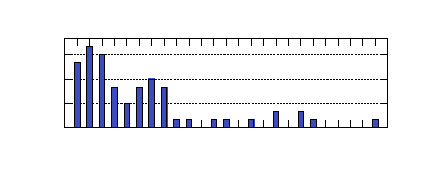
\includegraphics[width={194.00bp},height={90.60bp}]{images/std_accuracy_gamma_losses}}%
    \gplfronttext
  \end{picture}%
\endgroup
}}
\caption{Results on clustering loss impact across augmentation
steps and loss weight tuning.}
\label{fig:ablation-supp}
\end{figure}

\paragraph{Clustering loss ablation}
\tablename~\ref{tab:ablation} shows accuracy gains (Q1, median, Q3,
mean) for the full model and after removing the clustering loss on
102 UCR datasets. Without this loss,
ASCENSION$_{\text{ResNet-Emb}}$ drops from $2.1\%$ to $-0.05\%$,
and ASCENSION$_{\text{FCN-Emb}}$ from $1.2\%$ to $-0.05\%$.
Overlapping class distributions hinder discrimination, a known
effect in clustering-based methods like VaDE. As seen in
Figure~\ref{fig:ablation-supp}(a), performance also declines
progressively with each extra augmentation step.

\begin{table}[H]
\centering
\small
\caption{Average accuracy gains for the full model
(\textbf{Full}, no component removed) and after individually
removing $\alpha$-scaling or the clustering loss. Removing
$\alpha$-scaling yields at most a marginal gain ($\leq 0.4\%$). Removing the clustering loss yields a $-0.05\%$ drop,
confirming both components are essential for ASCENSION's
improvements.}
\label{tab:ablation}
\begin{tabular}{@{}llrrrr@{}}
\toprule
\textbf{Component removed} & \textbf{Classifier}
  & $\uparrow$Q1 & $\uparrow$Median & $\uparrow$Q3 & $\uparrow$Mean \\
\midrule
\multirow{2}{*}{$\alpha$-scaling mechanism}
  & ASCENSION$_{\text{ResNet-Emb}}$ & $-1.0\%$ & $0.2\%$  & $1.5\%$ & $0.09\%$ \\
  & ASCENSION$_{\text{FCN-Emb}}$    & $-0.4\%$ & $0.5\%$  & $2\%$   & $0.4\%$ \\
\midrule
\multirow{2}{*}{Clustering loss}
  & ASCENSION$_{\text{ResNet-Emb}}$ & $-1.5\%$ & $-0.8\%$ & $0.05\%$ & $-0.05\%$ \\
  & ASCENSION$_{\text{FCN-Emb}}$    & $-1.6\%$ & $-0.04\%$& $0.05\%$ & $-0.05\%$ \\
\midrule
\multirow{2}{*}{Full (no removal)}
  & ASCENSION$_{\text{ResNet-Emb}}$ & $0.03\%$ & $1.6\%$  & $3.6\%$  & $\mathbf{2.1\%}$ \\
  & ASCENSION$_{\text{FCN-Emb}}$    & $-0.02\%$& $0.05\%$ & $2\%$    & $\mathbf{1.2\%}$ \\
\bottomrule
\end{tabular}
\end{table}

\paragraph{Loss weight hyperparameter tuning}
Figure~\ref{fig:ablation-supp}(b) reports the average accuracy
variance over all loss-weight combinations examined for each
dataset. Across most datasets, accuracy remains stable regardless
of the specific choice of
$(\gamma_1, \gamma_2, \gamma_3, \gamma_4)$. Consequently, no
parameter tuning seems necessary and setting all weights
uniformly
($\gamma_1 = \gamma_2 = \gamma_3 = \gamma_4 = 1$) is a reasonable
choice.

\subsection{Ablation 2: Feature-based gain analysis}
\label{sec:analysis:features}

% REVISED FOR TMLR (rebuttal C2)
As shown in Section~\ref{sec:results:main}, ASCENSION compares
favourably to traditional and generative DA methods, but a
substantial share of datasets shows no gain or even degradation
(Unchanged/Worsened in \tablename~\ref{tab:main-results}; full
results in Appendix~\ref{app:per_dataset}). To pinpoint which
datasets benefit from DA, we perform a feature-based analysis,
computed on the fixed-configuration runs, using ASCENSION with
ResNet, FCN, and Moment as external classifiers for fair
comparison.

\paragraph{Feature extraction}
We use the 22 \textbf{CA}nonical \textbf{T}ime-series
\textbf{CH}aracteristics \citep[\texttt{catch22},][]{lubba2019catch22}
to featurise TS, and add two
additional features: (F23) the train/test split ratio, and (F24)
the distribution discrepancy ratio between train and test sets
(see metric definitions in Appendix~\ref{app:feature_risk}). A full
description of the 24 features (F1--F24) is provided in
Appendix~\ref{app:per_dataset}. F23 is computable from dataset
sizes and F24 requires the test set and is used here as a
post-hoc indicator.

\paragraph{Analysis methodology}
We average TS features per dataset to identify those
most and least responsive to augmentation. We then assess how DA
affects classification to pinpoint key influencing features. A
shallow random forest with a high number of estimators is used
to predict augmentation outcomes from the averaged F1--F24
features across DA methods. We repeat the protocol for ResNet,
FCN, and Moment.

\newcommand{\panelTag}[1]{\noindent\hspace*{0.5em}\textit{\small #1}\par\vspace{-2pt}}
\begin{figure}[!t]
\centering
\daLegendBlock\par\smallskip
% REVISED FOR TMLR (minor: figure spacing)
\panelTag{ResNet}\resizebox{\linewidth}{!}{\input{images/Resnet_Catch22_Histo.tex}}\\
\panelTag{FCN}\resizebox{\linewidth}{!}{% GNUPLOT: LaTeX picture with Postscript
\begingroup
  \makeatletter
  \providecommand\color[2][]{%
    \GenericError{(gnuplot) \space\space\space\@spaces}{%
      Package color not loaded in conjunction with
      terminal option `colourtext'%
    }{See the gnuplot documentation for explanation.%
    }{Either use 'blacktext' in gnuplot or load the package
      color.sty in LaTeX.}%
    \renewcommand\color[2][]{}%
  }%
  \providecommand\includegraphics[2][]{%
    \GenericError{(gnuplot) \space\space\space\@spaces}{%
      Package graphicx or graphics not loaded%
    }{See the gnuplot documentation for explanation.%
    }{The gnuplot epslatex terminal needs graphicx.sty or graphics.sty.}%
    \renewcommand\includegraphics[2][]{}%
  }%
  \providecommand\rotatebox[2]{#2}%
  \@ifundefined{ifGPcolor}{%
    \newif\ifGPcolor
    \GPcolorfalse
  }{}%
  \@ifundefined{ifGPblacktext}{%
    \newif\ifGPblacktext
    \GPblacktexttrue
  }{}%
  % define a \g@addto@macro without @ in the name:
  \let\gplgaddtomacro\g@addto@macro
  % define empty templates for all commands taking text:
  \gdef\gplbacktext{}%
  \gdef\gplfronttext{}%
  \makeatother
  \ifGPblacktext
    % no textcolor at all
    \def\colorrgb#1{}%
    \def\colorgray#1{}%
  \else
    % gray or color?
    \ifGPcolor
      \def\colorrgb#1{\color[rgb]{#1}}%
      \def\colorgray#1{\color[gray]{#1}}%
      \expandafter\def\csname LTw\endcsname{\color{white}}%
      \expandafter\def\csname LTb\endcsname{\color{black}}%
      \expandafter\def\csname LTa\endcsname{\color{black}}%
      \expandafter\def\csname LT0\endcsname{\color[rgb]{1,0,0}}%
      \expandafter\def\csname LT1\endcsname{\color[rgb]{0,1,0}}%
      \expandafter\def\csname LT2\endcsname{\color[rgb]{0,0,1}}%
      \expandafter\def\csname LT3\endcsname{\color[rgb]{1,0,1}}%
      \expandafter\def\csname LT4\endcsname{\color[rgb]{0,1,1}}%
      \expandafter\def\csname LT5\endcsname{\color[rgb]{1,1,0}}%
      \expandafter\def\csname LT6\endcsname{\color[rgb]{0,0,0}}%
      \expandafter\def\csname LT7\endcsname{\color[rgb]{1,0.3,0}}%
      \expandafter\def\csname LT8\endcsname{\color[rgb]{0.5,0.5,0.5}}%
    \else
      % gray
      \def\colorrgb#1{\color{black}}%
      \def\colorgray#1{\color[gray]{#1}}%
      \expandafter\def\csname LTw\endcsname{\color{white}}%
      \expandafter\def\csname LTb\endcsname{\color{black}}%
      \expandafter\def\csname LTa\endcsname{\color{black}}%
      \expandafter\def\csname LT0\endcsname{\color{black}}%
      \expandafter\def\csname LT1\endcsname{\color{black}}%
      \expandafter\def\csname LT2\endcsname{\color{black}}%
      \expandafter\def\csname LT3\endcsname{\color{black}}%
      \expandafter\def\csname LT4\endcsname{\color{black}}%
      \expandafter\def\csname LT5\endcsname{\color{black}}%
      \expandafter\def\csname LT6\endcsname{\color{black}}%
      \expandafter\def\csname LT7\endcsname{\color{black}}%
      \expandafter\def\csname LT8\endcsname{\color{black}}%
    \fi
  \fi
    \setlength{\unitlength}{0.0500bp}%
    \ifx\gptboxheight\undefined%
      \newlength{\gptboxheight}%
      \newlength{\gptboxwidth}%
      \newsavebox{\gptboxtext}%
    \fi%
    \setlength{\fboxrule}{0.5pt}%
    \setlength{\fboxsep}{1pt}%
    \definecolor{tbcol}{rgb}{1,1,1}%
\begin{picture}(8640.00,1512.00)%
    \gplgaddtomacro\gplbacktext{%
      \csname LTb\endcsname%%
     \put(-725,0){
      \put(800,440){\makebox(0,0)[r]{\strut{}\scriptsize$0$}}%
      \csname LTb\endcsname%%
      \put(800,625){\makebox(0,0)[r]{\strut{}\scriptsize$0.05$}}%
      \csname LTb\endcsname%%
      \put(800,810){\makebox(0,0)[r]{\strut{}\scriptsize$0.1$}}%
      \put(400,810){\makebox(0,0)[r]{\strut{}\scriptsize \rotatebox{90}{Importance}}}%
      \csname LTb\endcsname%%
      \put(800,996){\makebox(0,0)[r]{\strut{}\scriptsize$0.15$}}%
      \csname LTb\endcsname%%
      \put(800,1181){\makebox(0,0)[r]{\strut{}\scriptsize$0.2$}}%
      % \put(1153,300){\makebox(0,0){\strut{}\scriptsize F1}}%
      % \put(1449,300){\makebox(0,0){\strut{}\scriptsize F2}}%
      % \put(1744,300){\makebox(0,0){\strut{}\scriptsize F3}}%
      % \put(2039,300){\makebox(0,0){\strut{}\scriptsize F4}}%
      % \put(2335,300){\makebox(0,0){\strut{}\scriptsize F5}}%
      % \put(2630,300){\makebox(0,0){\strut{}\scriptsize F6}}%
      % \put(2926,300){\makebox(0,0){\strut{}\scriptsize F7}}%
      % \put(3221,300){\makebox(0,0){\strut{}\scriptsize F8}}%
      % \put(3516,300){\makebox(0,0){\strut{}\scriptsize F9}}%
      % \put(3812,300){\makebox(0,0){\strut{}\scriptsize F10}}%
      % \put(4107,300){\makebox(0,0){\strut{}\scriptsize F11}}%
      % \put(4402,300){\makebox(0,0){\strut{}\scriptsize F12}}%
      % \put(4698,300){\makebox(0,0){\strut{}\scriptsize F13}}%
      % \put(4993,300){\makebox(0,0){\strut{}\scriptsize F14}}%
      % \put(5288,300){\makebox(0,0){\strut{}\scriptsize F15}}%
      % \put(5584,300){\makebox(0,0){\strut{}\scriptsize F16}}%
      % \put(5879,300){\makebox(0,0){\strut{}\scriptsize F17}}%
      % \put(6174,300){\makebox(0,0){\strut{}\scriptsize F18}}%
      % \put(6470,300){\makebox(0,0){\strut{}\scriptsize F19}}%
      % \put(6765,300){\makebox(0,0){\strut{}\scriptsize F20}}%
      % \put(7061,300){\makebox(0,0){\strut{}\scriptsize F21}}%
      % \put(7356,300){\makebox(0,0){\strut{}\scriptsize F22}}%
      % \put(7651,300){\makebox(0,0){\strut{}\scriptsize F23}}%
      % \put(7947,300){\makebox(0,0){\strut{}\scriptsize F24}}%
      }
    }%
    \gplgaddtomacro\gplfronttext{%
    }%
    \gplbacktext
    \put(0,0){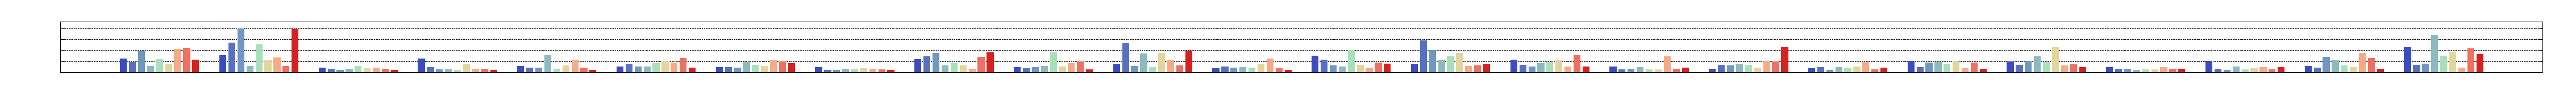
\includegraphics[width={432.00bp},height={75.60bp}]{images/FCN_Catch22_Histo}}%
    \gplfronttext
  \end{picture}%
\endgroup
}\\
\panelTag{Moment}\resizebox{\linewidth}{!}{\input{images/Moment_Catch22_Histo.tex}}
\caption{Feature importance over 24 features (F1--F24, see
Appendix~\ref{app:feature_risk}). Key ones include F2: top
$z$-score range, F14: mean time between extreme events, F20:
slow fluctuations, F23: train/test size ratio, F24: train--test
distribution discrepancy (Appendix~\ref{app:discrepancy}).}
\label{fig:catch22-importance}
\end{figure}

\paragraph{Results}
Figure~\ref{fig:catch22-importance} shows that each DA method
aligns with specific dataset features depending on the
classifier. For ResNet/FCN, VaDE links to F2 (high $z$-score
frequency), F11 (2D distance change), and F17 (longest decreasing
trend). Diffusion-TS to F14 (rapid fluctuations); Time-DDPM
(ResNet) to F20 (slow fluctuations); and ASCENSION to F24
(train--test distribution gap). With Moment, feature rankings
% TODO(number): re-verify on fixed-config Figure 5 regeneration
shift: F15 (rapid fluctuations) peaks sharply ($0.64$ for
Diffusion-TS, $0.54$ for TTS-GAN), while ASCENSION depends less
on F24, and VaDE more, showing that pretraining reshapes which
dataset traits drive augmentation gains.
\label{sec:analysis:discrepancy}
To investigate the discrepancy axis directly, we sort the $102$
UCR datasets by ascending discrepancy
(F24, Appendix~\ref{app:discrepancy}) and report the cumulative
mean accuracy gain as datasets are added in this order
(Figure~\ref{fig:cumsum-disc}).

\begin{figure}[!t]
\centering
% REVISED FOR TMLR (minor: figure spacing)
\daLegendBlock\par\smallskip
\resizebox{\linewidth}{!}{% GNUPLOT: LaTeX picture with Postscript
\begingroup
\providecommand{\xticRot}{-90}
\providecommand{\xticOffset}{3pt}
\providecommand{\xticSize}{4.25pt}
  \makeatletter
  \providecommand\color[2][]{%
    \GenericError{(gnuplot) \space\space\space\@spaces}{%
      Package color not loaded in conjunction with
      terminal option `colourtext'%
    }{See the gnuplot documentation for explanation.%
    }{Either use 'blacktext' in gnuplot or load the package
      color.sty in LaTeX.}%
    \renewcommand\color[2][]{}%
  }%
  \providecommand\includegraphics[2][]{%
    \GenericError{(gnuplot) \space\space\space\@spaces}{%
      Package graphicx or graphics not loaded%
    }{See the gnuplot documentation for explanation.%
    }{The gnuplot epslatex terminal needs graphicx.sty or graphics.sty.}%
    \renewcommand\includegraphics[2][]{}%
  }%
  \providecommand\rotatebox[2]{#2}%
  \@ifundefined{ifGPcolor}{%
    \newif\ifGPcolor
    \GPcolortrue
  }{}%
  \@ifundefined{ifGPblacktext}{%
    \newif\ifGPblacktext
    \GPblacktexttrue
  }{}%
  % define a \g@addto@macro without @ in the name:
  \let\gplgaddtomacro\g@addto@macro
  % define empty templates for all commands taking text:
  \gdef\gplbacktext{}%
  \gdef\gplfronttext{}%
  \makeatother
  \ifGPblacktext
    % no textcolor at all
    \def\colorrgb#1{}%
    \def\colorgray#1{}%
  \else
    % gray or color?
    \ifGPcolor
      \def\colorrgb#1{\color[rgb]{#1}}%
      \def\colorgray#1{\color[gray]{#1}}%
      \expandafter\def\csname LTw\endcsname{\color{white}}%
      \expandafter\def\csname LTb\endcsname{\color{black}}%
      \expandafter\def\csname LTa\endcsname{\color{black}}%
      \expandafter\def\csname LT0\endcsname{\color[rgb]{1,0,0}}%
      \expandafter\def\csname LT1\endcsname{\color[rgb]{0,1,0}}%
      \expandafter\def\csname LT2\endcsname{\color[rgb]{0,0,1}}%
      \expandafter\def\csname LT3\endcsname{\color[rgb]{1,0,1}}%
      \expandafter\def\csname LT4\endcsname{\color[rgb]{0,1,1}}%
      \expandafter\def\csname LT5\endcsname{\color[rgb]{1,1,0}}%
      \expandafter\def\csname LT6\endcsname{\color[rgb]{0,0,0}}%
      \expandafter\def\csname LT7\endcsname{\color[rgb]{1,0.3,0}}%
      \expandafter\def\csname LT8\endcsname{\color[rgb]{0.5,0.5,0.5}}%
    \else
      % gray
      \def\colorrgb#1{\color{black}}%
      \def\colorgray#1{\color[gray]{#1}}%
      \expandafter\def\csname LTw\endcsname{\color{white}}%
      \expandafter\def\csname LTb\endcsname{\color{black}}%
      \expandafter\def\csname LTa\endcsname{\color{black}}%
      \expandafter\def\csname LT0\endcsname{\color{black}}%
      \expandafter\def\csname LT1\endcsname{\color{black}}%
      \expandafter\def\csname LT2\endcsname{\color{black}}%
      \expandafter\def\csname LT3\endcsname{\color{black}}%
      \expandafter\def\csname LT4\endcsname{\color{black}}%
      \expandafter\def\csname LT5\endcsname{\color{black}}%
      \expandafter\def\csname LT6\endcsname{\color{black}}%
      \expandafter\def\csname LT7\endcsname{\color{black}}%
      \expandafter\def\csname LT8\endcsname{\color{black}}%
    \fi
  \fi
    \setlength{\unitlength}{0.0500bp}%
    \ifx\gptboxheight\undefined%
      \newlength{\gptboxheight}%
      \newlength{\gptboxwidth}%
      \newsavebox{\gptboxtext}%
    \fi%
    \setlength{\fboxrule}{0.5pt}%
    \setlength{\fboxsep}{1pt}%
    \definecolor{tbcol}{rgb}{1,1,1}%
\begin{picture}(8640.00,3024.00)%
    \gplgaddtomacro\gplbacktext{%
      \csname LTb\endcsname%%
      \put(462,880){\makebox(0,0)[r]{\strut{}$-8$}}%
      \csname LTb\endcsname%%
      \put(462,1230){\makebox(0,0)[r]{\strut{}$-6$}}%
      \csname LTb\endcsname%%
      \put(462,1579){\makebox(0,0)[r]{\strut{}$-4$}}%
      \csname LTb\endcsname%%
      \put(462,1929){\makebox(0,0)[r]{\strut{}$-2$}}%
      \csname LTb\endcsname%%
      \put(462,2279){\makebox(0,0)[r]{\strut{}$0$}}%
      \csname LTb\endcsname%%
      \put(462,2628){\makebox(0,0)[r]{\strut{}$2$}}%
      \put(668,858){\raisebox{-\xticOffset}{\rotatebox{\xticRot}{\makebox(0,0)[l]{\fontsize{\xticSize}{4pt}\selectfont \strut{}D39}}}}%
      \put(743,858){\raisebox{-\xticOffset}{\rotatebox{\xticRot}{\makebox(0,0)[l]{\fontsize{\xticSize}{4pt}\selectfont \strut{}D22}}}}%
      \put(817,858){\raisebox{-\xticOffset}{\rotatebox{\xticRot}{\makebox(0,0)[l]{\fontsize{\xticSize}{4pt}\selectfont \strut{}D55}}}}%
      \put(891,858){\raisebox{-\xticOffset}{\rotatebox{\xticRot}{\makebox(0,0)[l]{\fontsize{\xticSize}{4pt}\selectfont \strut{}D68}}}}%
      \put(965,858){\raisebox{-\xticOffset}{\rotatebox{\xticRot}{\makebox(0,0)[l]{\fontsize{\xticSize}{4pt}\selectfont \strut{}D25}}}}%
      \put(1040,858){\raisebox{-\xticOffset}{\rotatebox{\xticRot}{\makebox(0,0)[l]{\fontsize{\xticSize}{4pt}\selectfont \strut{}D98}}}}%
      \put(1114,858){\raisebox{-\xticOffset}{\rotatebox{\xticRot}{\makebox(0,0)[l]{\fontsize{\xticSize}{4pt}\selectfont \strut{}D89}}}}%
      \put(1188,858){\raisebox{-\xticOffset}{\rotatebox{\xticRot}{\makebox(0,0)[l]{\fontsize{\xticSize}{4pt}\selectfont \strut{}D72}}}}%
      \put(1262,858){\raisebox{-\xticOffset}{\rotatebox{\xticRot}{\makebox(0,0)[l]{\fontsize{\xticSize}{4pt}\selectfont \strut{}D6}}}}%
      \put(1337,858){\raisebox{-\xticOffset}{\rotatebox{\xticRot}{\makebox(0,0)[l]{\fontsize{\xticSize}{4pt}\selectfont \strut{}D100}}}}%
      \put(1411,858){\raisebox{-\xticOffset}{\rotatebox{\xticRot}{\makebox(0,0)[l]{\fontsize{\xticSize}{4pt}\selectfont \strut{}D83}}}}%
      \put(1485,858){\raisebox{-\xticOffset}{\rotatebox{\xticRot}{\makebox(0,0)[l]{\fontsize{\xticSize}{4pt}\selectfont \strut{}D63}}}}%
      \put(1559,858){\raisebox{-\xticOffset}{\rotatebox{\xticRot}{\makebox(0,0)[l]{\fontsize{\xticSize}{4pt}\selectfont \strut{}D101}}}}%
      \put(1634,858){\raisebox{-\xticOffset}{\rotatebox{\xticRot}{\makebox(0,0)[l]{\fontsize{\xticSize}{4pt}\selectfont \strut{}D5}}}}%
      \put(1708,858){\raisebox{-\xticOffset}{\rotatebox{\xticRot}{\makebox(0,0)[l]{\fontsize{\xticSize}{4pt}\selectfont \strut{}D77}}}}%
      \put(1782,858){\raisebox{-\xticOffset}{\rotatebox{\xticRot}{\makebox(0,0)[l]{\fontsize{\xticSize}{4pt}\selectfont \strut{}D67}}}}%
      \put(1856,858){\raisebox{-\xticOffset}{\rotatebox{\xticRot}{\makebox(0,0)[l]{\fontsize{\xticSize}{4pt}\selectfont \strut{}D50}}}}%
      \put(1931,858){\raisebox{-\xticOffset}{\rotatebox{\xticRot}{\makebox(0,0)[l]{\fontsize{\xticSize}{4pt}\selectfont \strut{}D65}}}}%
      \put(2005,858){\raisebox{-\xticOffset}{\rotatebox{\xticRot}{\makebox(0,0)[l]{\fontsize{\xticSize}{4pt}\selectfont \strut{}D56}}}}%
      \put(2079,858){\raisebox{-\xticOffset}{\rotatebox{\xticRot}{\makebox(0,0)[l]{\fontsize{\xticSize}{4pt}\selectfont \strut{}D52}}}}%
      \put(2153,858){\raisebox{-\xticOffset}{\rotatebox{\xticRot}{\makebox(0,0)[l]{\fontsize{\xticSize}{4pt}\selectfont \strut{}D69}}}}%
      \put(2228,858){\raisebox{-\xticOffset}{\rotatebox{\xticRot}{\makebox(0,0)[l]{\fontsize{\xticSize}{4pt}\selectfont \strut{}D47}}}}%
      \put(2302,858){\raisebox{-\xticOffset}{\rotatebox{\xticRot}{\makebox(0,0)[l]{\fontsize{\xticSize}{4pt}\selectfont \strut{}D75}}}}%
      \put(2376,858){\raisebox{-\xticOffset}{\rotatebox{\xticRot}{\makebox(0,0)[l]{\fontsize{\xticSize}{4pt}\selectfont \strut{}D64}}}}%
      \put(2450,858){\raisebox{-\xticOffset}{\rotatebox{\xticRot}{\makebox(0,0)[l]{\fontsize{\xticSize}{4pt}\selectfont \strut{}D1}}}}%
      \put(2525,858){\raisebox{-\xticOffset}{\rotatebox{\xticRot}{\makebox(0,0)[l]{\fontsize{\xticSize}{4pt}\selectfont \strut{}D59}}}}%
      \put(2599,858){\raisebox{-\xticOffset}{\rotatebox{\xticRot}{\makebox(0,0)[l]{\fontsize{\xticSize}{4pt}\selectfont \strut{}D16}}}}%
      \put(2673,858){\raisebox{-\xticOffset}{\rotatebox{\xticRot}{\makebox(0,0)[l]{\fontsize{\xticSize}{4pt}\selectfont \strut{}D84}}}}%
      \put(2747,858){\raisebox{-\xticOffset}{\rotatebox{\xticRot}{\makebox(0,0)[l]{\fontsize{\xticSize}{4pt}\selectfont \strut{}D88}}}}%
      \put(2822,858){\raisebox{-\xticOffset}{\rotatebox{\xticRot}{\makebox(0,0)[l]{\fontsize{\xticSize}{4pt}\selectfont \strut{}D92}}}}%
      \put(2896,858){\raisebox{-\xticOffset}{\rotatebox{\xticRot}{\makebox(0,0)[l]{\fontsize{\xticSize}{4pt}\selectfont \strut{}D61}}}}%
      \put(2970,858){\raisebox{-\xticOffset}{\rotatebox{\xticRot}{\makebox(0,0)[l]{\fontsize{\xticSize}{4pt}\selectfont \strut{}D73}}}}%
      \put(3044,858){\raisebox{-\xticOffset}{\rotatebox{\xticRot}{\makebox(0,0)[l]{\fontsize{\xticSize}{4pt}\selectfont \strut{}D26}}}}%
      \put(3119,858){\raisebox{-\xticOffset}{\rotatebox{\xticRot}{\makebox(0,0)[l]{\fontsize{\xticSize}{4pt}\selectfont \strut{}D13}}}}%
      \put(3193,858){\raisebox{-\xticOffset}{\rotatebox{\xticRot}{\makebox(0,0)[l]{\fontsize{\xticSize}{4pt}\selectfont \strut{}D62}}}}%
      \put(3267,858){\raisebox{-\xticOffset}{\rotatebox{\xticRot}{\makebox(0,0)[l]{\fontsize{\xticSize}{4pt}\selectfont \strut{}D60}}}}%
      \put(3341,858){\raisebox{-\xticOffset}{\rotatebox{\xticRot}{\makebox(0,0)[l]{\fontsize{\xticSize}{4pt}\selectfont \strut{}D31}}}}%
      \put(3416,858){\raisebox{-\xticOffset}{\rotatebox{\xticRot}{\makebox(0,0)[l]{\fontsize{\xticSize}{4pt}\selectfont \strut{}D57}}}}%
      \put(3490,858){\raisebox{-\xticOffset}{\rotatebox{\xticRot}{\makebox(0,0)[l]{\fontsize{\xticSize}{4pt}\selectfont \strut{}D42}}}}%
      \put(3564,858){\raisebox{-\xticOffset}{\rotatebox{\xticRot}{\makebox(0,0)[l]{\fontsize{\xticSize}{4pt}\selectfont \strut{}D78}}}}%
      \put(3638,858){\raisebox{-\xticOffset}{\rotatebox{\xticRot}{\makebox(0,0)[l]{\fontsize{\xticSize}{4pt}\selectfont \strut{}D30}}}}%
      \put(3713,858){\raisebox{-\xticOffset}{\rotatebox{\xticRot}{\makebox(0,0)[l]{\fontsize{\xticSize}{4pt}\selectfont \strut{}D80}}}}%
      \put(3787,858){\raisebox{-\xticOffset}{\rotatebox{\xticRot}{\makebox(0,0)[l]{\fontsize{\xticSize}{4pt}\selectfont \strut{}D74}}}}%
      \put(3861,858){\raisebox{-\xticOffset}{\rotatebox{\xticRot}{\makebox(0,0)[l]{\fontsize{\xticSize}{4pt}\selectfont \strut{}D35}}}}%
      \put(3935,858){\raisebox{-\xticOffset}{\rotatebox{\xticRot}{\makebox(0,0)[l]{\fontsize{\xticSize}{4pt}\selectfont \strut{}D90}}}}%
      \put(4010,858){\raisebox{-\xticOffset}{\rotatebox{\xticRot}{\makebox(0,0)[l]{\fontsize{\xticSize}{4pt}\selectfont \strut{}D29}}}}%
      \put(4084,858){\raisebox{-\xticOffset}{\rotatebox{\xticRot}{\makebox(0,0)[l]{\fontsize{\xticSize}{4pt}\selectfont \strut{}D53}}}}%
      \put(4158,858){\raisebox{-\xticOffset}{\rotatebox{\xticRot}{\makebox(0,0)[l]{\fontsize{\xticSize}{4pt}\selectfont \strut{}D23}}}}%
      \put(4232,858){\raisebox{-\xticOffset}{\rotatebox{\xticRot}{\makebox(0,0)[l]{\fontsize{\xticSize}{4pt}\selectfont \strut{}D14}}}}%
      \put(4307,858){\raisebox{-\xticOffset}{\rotatebox{\xticRot}{\makebox(0,0)[l]{\fontsize{\xticSize}{4pt}\selectfont \strut{}D91}}}}%
      \put(4381,858){\raisebox{-\xticOffset}{\rotatebox{\xticRot}{\makebox(0,0)[l]{\fontsize{\xticSize}{4pt}\selectfont \strut{}D48}}}}%
      \put(4455,858){\raisebox{-\xticOffset}{\rotatebox{\xticRot}{\makebox(0,0)[l]{\fontsize{\xticSize}{4pt}\selectfont \strut{}D32}}}}%
      \put(4529,858){\raisebox{-\xticOffset}{\rotatebox{\xticRot}{\makebox(0,0)[l]{\fontsize{\xticSize}{4pt}\selectfont \strut{}D20}}}}%
      \put(4604,858){\raisebox{-\xticOffset}{\rotatebox{\xticRot}{\makebox(0,0)[l]{\fontsize{\xticSize}{4pt}\selectfont \strut{}D41}}}}%
      \put(4678,858){\raisebox{-\xticOffset}{\rotatebox{\xticRot}{\makebox(0,0)[l]{\fontsize{\xticSize}{4pt}\selectfont \strut{}D37}}}}%
      \put(4752,858){\raisebox{-\xticOffset}{\rotatebox{\xticRot}{\makebox(0,0)[l]{\fontsize{\xticSize}{4pt}\selectfont \strut{}D86}}}}%
      \put(4826,858){\raisebox{-\xticOffset}{\rotatebox{\xticRot}{\makebox(0,0)[l]{\fontsize{\xticSize}{4pt}\selectfont \strut{}D94}}}}%
      \put(4901,858){\raisebox{-\xticOffset}{\rotatebox{\xticRot}{\makebox(0,0)[l]{\fontsize{\xticSize}{4pt}\selectfont \strut{}D49}}}}%
      \put(4975,858){\raisebox{-\xticOffset}{\rotatebox{\xticRot}{\makebox(0,0)[l]{\fontsize{\xticSize}{4pt}\selectfont \strut{}D66}}}}%
      \put(5049,858){\raisebox{-\xticOffset}{\rotatebox{\xticRot}{\makebox(0,0)[l]{\fontsize{\xticSize}{4pt}\selectfont \strut{}D36}}}}%
      \put(5123,858){\raisebox{-\xticOffset}{\rotatebox{\xticRot}{\makebox(0,0)[l]{\fontsize{\xticSize}{4pt}\selectfont \strut{}D102}}}}%
      \put(5198,858){\raisebox{-\xticOffset}{\rotatebox{\xticRot}{\makebox(0,0)[l]{\fontsize{\xticSize}{4pt}\selectfont \strut{}D93}}}}%
      \put(5272,858){\raisebox{-\xticOffset}{\rotatebox{\xticRot}{\makebox(0,0)[l]{\fontsize{\xticSize}{4pt}\selectfont \strut{}D17}}}}%
      \put(5346,858){\raisebox{-\xticOffset}{\rotatebox{\xticRot}{\makebox(0,0)[l]{\fontsize{\xticSize}{4pt}\selectfont \strut{}D34}}}}%
      \put(5420,858){\raisebox{-\xticOffset}{\rotatebox{\xticRot}{\makebox(0,0)[l]{\fontsize{\xticSize}{4pt}\selectfont \strut{}D79}}}}%
      \put(5495,858){\raisebox{-\xticOffset}{\rotatebox{\xticRot}{\makebox(0,0)[l]{\fontsize{\xticSize}{4pt}\selectfont \strut{}D27}}}}%
      \put(5569,858){\raisebox{-\xticOffset}{\rotatebox{\xticRot}{\makebox(0,0)[l]{\fontsize{\xticSize}{4pt}\selectfont \strut{}D82}}}}%
      \put(5643,858){\raisebox{-\xticOffset}{\rotatebox{\xticRot}{\makebox(0,0)[l]{\fontsize{\xticSize}{4pt}\selectfont \strut{}D95}}}}%
      \put(5717,858){\raisebox{-\xticOffset}{\rotatebox{\xticRot}{\makebox(0,0)[l]{\fontsize{\xticSize}{4pt}\selectfont \strut{}D10}}}}%
      \put(5792,858){\raisebox{-\xticOffset}{\rotatebox{\xticRot}{\makebox(0,0)[l]{\fontsize{\xticSize}{4pt}\selectfont \strut{}D70}}}}%
      \put(5866,858){\raisebox{-\xticOffset}{\rotatebox{\xticRot}{\makebox(0,0)[l]{\fontsize{\xticSize}{4pt}\selectfont \strut{}D96}}}}%
      \put(5940,858){\raisebox{-\xticOffset}{\rotatebox{\xticRot}{\makebox(0,0)[l]{\fontsize{\xticSize}{4pt}\selectfont \strut{}D44}}}}%
      \put(6014,858){\raisebox{-\xticOffset}{\rotatebox{\xticRot}{\makebox(0,0)[l]{\fontsize{\xticSize}{4pt}\selectfont \strut{}D43}}}}%
      \put(6089,858){\raisebox{-\xticOffset}{\rotatebox{\xticRot}{\makebox(0,0)[l]{\fontsize{\xticSize}{4pt}\selectfont \strut{}D12}}}}%
      \put(6163,858){\raisebox{-\xticOffset}{\rotatebox{\xticRot}{\makebox(0,0)[l]{\fontsize{\xticSize}{4pt}\selectfont \strut{}D38}}}}%
      \put(6237,858){\raisebox{-\xticOffset}{\rotatebox{\xticRot}{\makebox(0,0)[l]{\fontsize{\xticSize}{4pt}\selectfont \strut{}D40}}}}%
      \put(6311,858){\raisebox{-\xticOffset}{\rotatebox{\xticRot}{\makebox(0,0)[l]{\fontsize{\xticSize}{4pt}\selectfont \strut{}D2}}}}%
      \put(6386,858){\raisebox{-\xticOffset}{\rotatebox{\xticRot}{\makebox(0,0)[l]{\fontsize{\xticSize}{4pt}\selectfont \strut{}D9}}}}%
      \put(6460,858){\raisebox{-\xticOffset}{\rotatebox{\xticRot}{\makebox(0,0)[l]{\fontsize{\xticSize}{4pt}\selectfont \strut{}D46}}}}%
      \put(6534,858){\raisebox{-\xticOffset}{\rotatebox{\xticRot}{\makebox(0,0)[l]{\fontsize{\xticSize}{4pt}\selectfont \strut{}D24}}}}%
      \put(6608,858){\raisebox{-\xticOffset}{\rotatebox{\xticRot}{\makebox(0,0)[l]{\fontsize{\xticSize}{4pt}\selectfont \strut{}D33}}}}%
      \put(6683,858){\raisebox{-\xticOffset}{\rotatebox{\xticRot}{\makebox(0,0)[l]{\fontsize{\xticSize}{4pt}\selectfont \strut{}D51}}}}%
      \put(6757,858){\raisebox{-\xticOffset}{\rotatebox{\xticRot}{\makebox(0,0)[l]{\fontsize{\xticSize}{4pt}\selectfont \strut{}D99}}}}%
      \put(6831,858){\raisebox{-\xticOffset}{\rotatebox{\xticRot}{\makebox(0,0)[l]{\fontsize{\xticSize}{4pt}\selectfont \strut{}D28}}}}%
      \put(6905,858){\raisebox{-\xticOffset}{\rotatebox{\xticRot}{\makebox(0,0)[l]{\fontsize{\xticSize}{4pt}\selectfont \strut{}D97}}}}%
      \put(6980,858){\raisebox{-\xticOffset}{\rotatebox{\xticRot}{\makebox(0,0)[l]{\fontsize{\xticSize}{4pt}\selectfont \strut{}D54}}}}%
      \put(7054,858){\raisebox{-\xticOffset}{\rotatebox{\xticRot}{\makebox(0,0)[l]{\fontsize{\xticSize}{4pt}\selectfont \strut{}D4}}}}%
      \put(7128,858){\raisebox{-\xticOffset}{\rotatebox{\xticRot}{\makebox(0,0)[l]{\fontsize{\xticSize}{4pt}\selectfont \strut{}D76}}}}%
      \put(7202,858){\raisebox{-\xticOffset}{\rotatebox{\xticRot}{\makebox(0,0)[l]{\fontsize{\xticSize}{4pt}\selectfont \strut{}D3}}}}%
      \put(7277,858){\raisebox{-\xticOffset}{\rotatebox{\xticRot}{\makebox(0,0)[l]{\fontsize{\xticSize}{4pt}\selectfont \strut{}D87}}}}%
      \put(7351,858){\raisebox{-\xticOffset}{\rotatebox{\xticRot}{\makebox(0,0)[l]{\fontsize{\xticSize}{4pt}\selectfont \strut{}D21}}}}%
      \put(7425,858){\raisebox{-\xticOffset}{\rotatebox{\xticRot}{\makebox(0,0)[l]{\fontsize{\xticSize}{4pt}\selectfont \strut{}D81}}}}%
      \put(7499,858){\raisebox{-\xticOffset}{\rotatebox{\xticRot}{\makebox(0,0)[l]{\fontsize{\xticSize}{4pt}\selectfont \strut{}D58}}}}%
      \put(7574,858){\raisebox{-\xticOffset}{\rotatebox{\xticRot}{\makebox(0,0)[l]{\fontsize{\xticSize}{4pt}\selectfont \strut{}D19}}}}%
      \put(7648,858){\raisebox{-\xticOffset}{\rotatebox{\xticRot}{\makebox(0,0)[l]{\fontsize{\xticSize}{4pt}\selectfont \strut{}D15}}}}%
      \put(7722,858){\raisebox{-\xticOffset}{\rotatebox{\xticRot}{\makebox(0,0)[l]{\fontsize{\xticSize}{4pt}\selectfont \strut{}D18}}}}%
      \put(7796,858){\raisebox{-\xticOffset}{\rotatebox{\xticRot}{\makebox(0,0)[l]{\fontsize{\xticSize}{4pt}\selectfont \strut{}D11}}}}%
      \put(7871,858){\raisebox{-\xticOffset}{\rotatebox{\xticRot}{\makebox(0,0)[l]{\fontsize{\xticSize}{4pt}\selectfont \strut{}D45}}}}%
      \put(7945,858){\raisebox{-\xticOffset}{\rotatebox{\xticRot}{\makebox(0,0)[l]{\fontsize{\xticSize}{4pt}\selectfont \strut{}D71}}}}%
      \put(8019,858){\raisebox{-\xticOffset}{\rotatebox{\xticRot}{\makebox(0,0)[l]{\fontsize{\xticSize}{4pt}\selectfont \strut{}D7}}}}%
      \put(8093,858){\raisebox{-\xticOffset}{\rotatebox{\xticRot}{\makebox(0,0)[l]{\fontsize{\xticSize}{4pt}\selectfont \strut{}D8}}}}%
      \put(8168,858){\raisebox{-\xticOffset}{\rotatebox{\xticRot}{\makebox(0,0)[l]{\fontsize{\xticSize}{4pt}\selectfont \strut{}D85}}}}%
    }%
    \gplgaddtomacro\gplfronttext{%
      \csname LTb\endcsname%%
      \put(747,2649){\makebox(0,0)[l]{\strut{}ResNet}}%
    }%
    \gplbacktext
    \put(0,0){
\includegraphics[width={432.00bp},height={151.20bp}]{cumulative_sum_discrepency_resnet}}%
    \gplfronttext
  \end{picture}%
\endgroup
}\\
\resizebox{\linewidth}{!}{\input{images/cumulative_sum_discrepancy_fcn.tex}}\\
\resizebox{\linewidth}{!}{\input{images/cumulative_sum_discrepancy_moment.tex}}

\caption{Cumulative accuracy improvement (\%) vs.\ F24
(train--test distribution discrepancy; see
\tablename~\ref{app:datasets}). Datasets are sorted by increasing
discrepancy. Per-dataset gains are averaged over the three
fixed-configuration runs.}
\label{fig:cumsum-disc}
\end{figure}
% \vspace{-12pt}

% REVISED FOR TMLR (rebuttal C2; curves regenerated on the fixed
% configuration, per-dataset gains averaged over the three runs)
ASCENSION's cumulative curve ends positive in eight of the nine
classifier-run combinations, while 65 of the 72 baseline curves end
negative. Crucially, the gap between ASCENSION and
the strongest generative baseline does not close on the
high-discrepancy datasets, \textit{i.e.}, where
in-distribution generative augmentation cannot help. This
robustness across the full discrepancy range, not concentration
in any one quartile, validates our central hypothesis:
progressive expansion into under-represented latent regions
yields beneficial augmentations \emph{regardless} of whether the
test distribution differs from training.

% -----------------------------------------------------------------
% Ablation 3 (Empirical acceptance rate / qualitative confidence
% study) was moved to Appendix~\ref{sec:analysis:confidence} as a
% robustness check.  The Prop 1 connection is already established
% by Ablation 1 (clustering-loss ablation), so the boxplot did not
% earn its place in the main paper.
% -----------------------------------------------------------------

% Per-macro-domain breakdown lives in App. I
% (\tablename s~\ref{Tab:Macro_ResNet}--\ref{Tab:Macro_Moment}); not
% promoted to the main paper.
